\chapter{Simulation results for generating arbitrary waveform signals}
The \gls{ab:dac} created in the previous chapter should be able to create various arbitrary waveform signals.
 To validate the used approach a harmonic balance simulation is used with the design tool \gls{ab:ads}.
  With this simulation it is possible to plot the voltage amplitude across the load impedance in the time domain.
   The harmonic balance simulation has the advantage that the whole system is modelled in a steady state mode, so no transient processes effect the simulation.
    It is important to note that the whole simulations are done under ideal conditions, hence no capacitances nor inductances of the conductors are considered.
     This is due to the fact, that the exact calculation of the bonds etc. is beyond the scope of this thesis.
The transistor model \gls{ab:hemt} (IAF GE MSL A204/IAF GaN25 HEMT CS LS SHfull) used in \gls{ab:ads} were modelled at the \gls{ab:iaf}.
Some signals are stated exemplary in the following.\\
All the simulation results have the same \gls{ab:osr} in common.
The \gls{ab:osr} is four and hence, due to the Nyquist-Shannon theorem, the sampling frequency is eight times the signal frequency.
This in mind, tuning the sampling frequency will result in tuning the signal frequency. \textbf{bandwidth limitation}
\textit{The lower bound is determined by the sampling time (inverse of the sampling frequency) and the smallest current achieved with the dimensioned transistors.
 The smallest achievable current times the smallest sampling time (highest sampling frequency) determine the smallest absolute slope achievable. \\
 \textbf{Is every signal possible to create?$\rightarrow$ a rect signal has too steep flanks to create. The signal bandwidth ranges from DC to 6 GHz but what is the amplitude range? Is there a limitation regarding the amplitude?}
\\
The smallest current is determined by the dimension of the transistor, which drives into saturation. 
The smallest saturated current is determined by the push-pull transistor geometry, here: 532 mA.}

\section{Time signal simulation with optimized/idealized components}
 The signals described in this section were generated with the \gls{ab:dac} design in the previous chapter and its resolution of 3-bit. 
The component dimensions are optimized with respect to the output signal.  

\subsection{sine wave}
To generate a signal with the \gls{ab:dac} of course a digital bitsequence is needed. This bitsequence, named riemanncode, controls the switches of the corresponding riemannpump. In fact that no MATLAB algorithm exists which computes the riemanncode by minimizing the error of the two signals this is done by hand. In fig. \ref{fig:SineWaveCodeGeneration} a sine wave is approximated with the help of eight different slopes as mentioned earlier. With this slopes the riemanncode was generated. The sequence of slopes is the following: \textit{+7 +3 -3 -7 -7 -3 +3 +7}.\\

A theoretical created sine wave is compared to the synthesized sine wave with the riemann pump simulation. As seen in Figure \ref{fig:SineCompare} the synthesized signal is very close to the theoretical optimal. The deviation is very small hence the signal to noise ratio is very low. As in equation \ref{eq:SNR_RiemannPumpConversion} stated the snr is calculated.


 \begin{figure}[htb!]
   \centering
   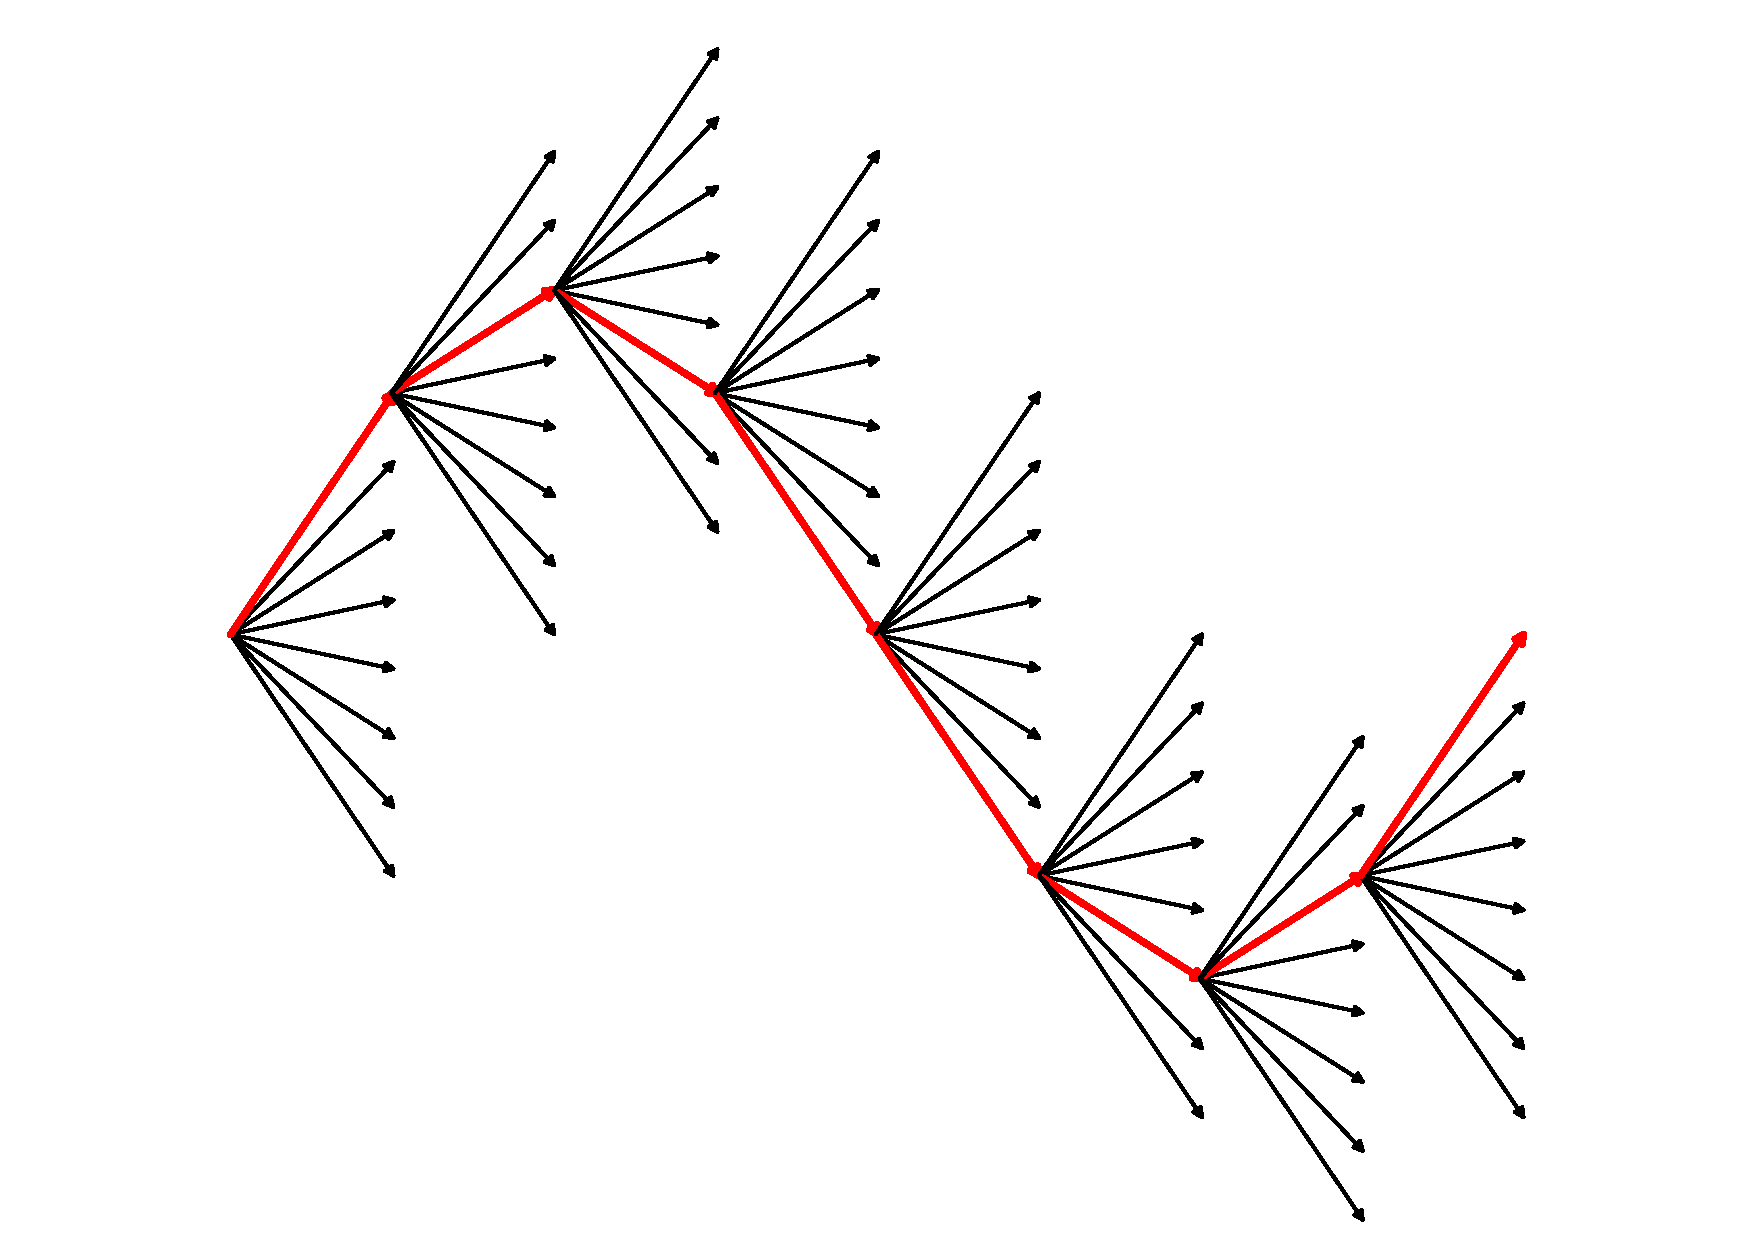
\includegraphics[width=1\textwidth]{RCgeneration_SineWave_byHand.pdf}
   \caption{Riemanncode generation for a sine wave by hand}
   \label{fig:SineWaveCodeGeneration}
\end{figure}
The corresponding riemanncode of fig \ref{fig:SineWaveCodeGeneration} to control the switches is: 000 010 101 111 111 101 010 000.\\
With this riemanncode a few more signals with different frequencies are simulated.

\begin{figure}[htb!]
   \centering
   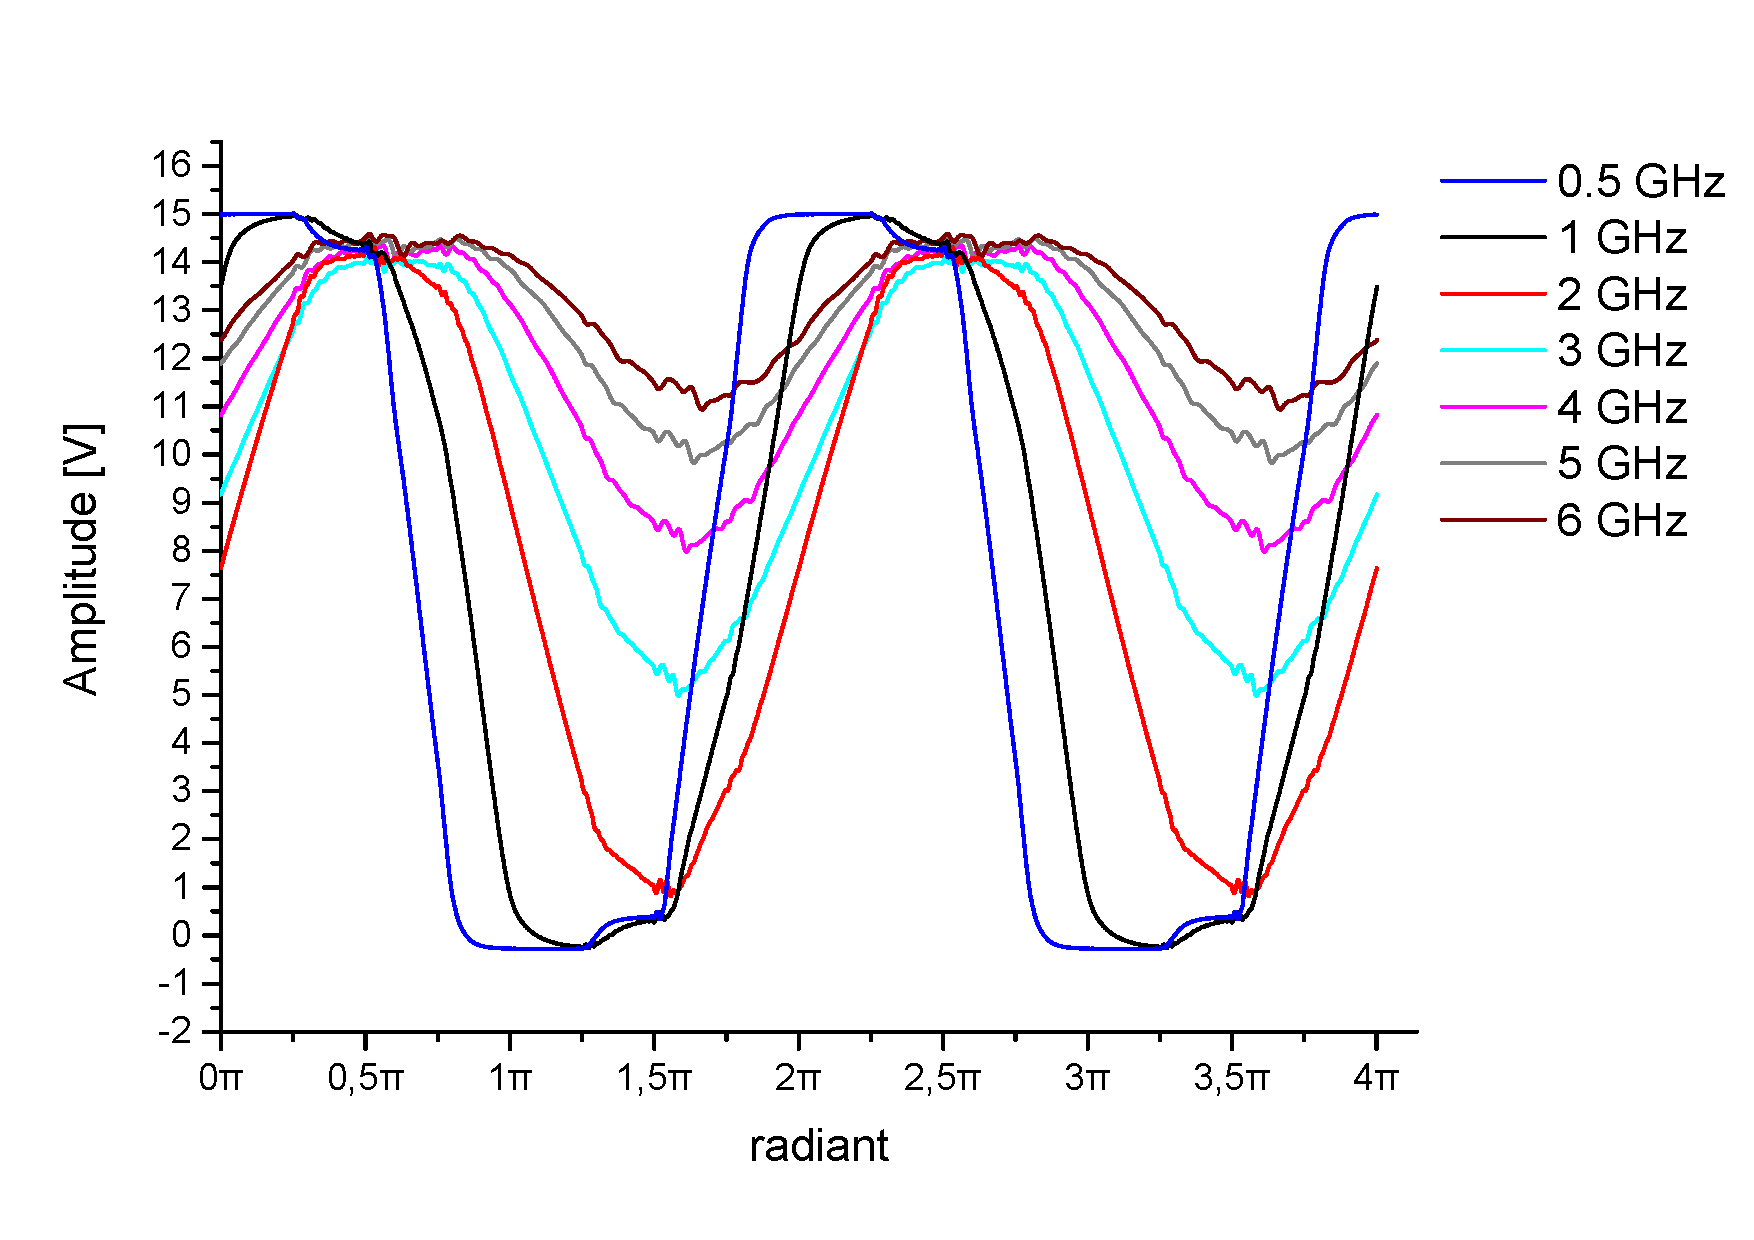
\includegraphics[width=0.75\textwidth]{Vout_sine_7signals_inOne_3bit_osr4.pdf}
   \caption{Signals based on the riemann code in fig \ref{fig:SineWaveCodeGeneration}}
   \label{fig:SineWavesGeneration}
\end{figure}
 
\begin{figure}[htb!]
   \centering
   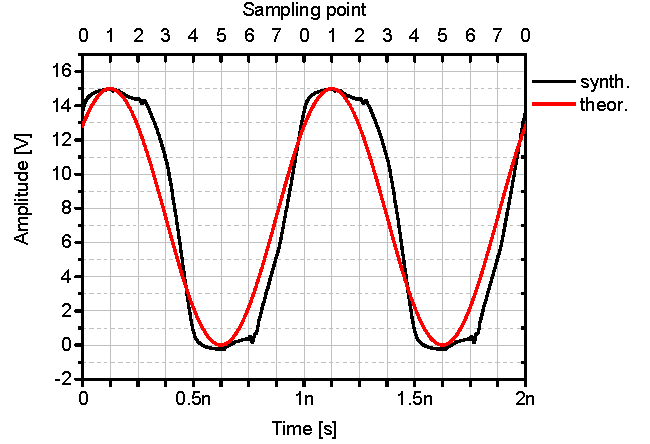
\includegraphics[width=0.75\textwidth]{Vout_SynthVsTheo.pdf}
   \caption{Synthesized sine wave with the theoretical sine wave}
   \label{fig:SineWaveSynthVsTheoretical}
\end{figure}
In fig. \ref{fig:SineWaveSynthVsTheoretical} the following signal is generated:
\begin{equation}
v(t)= \widehat{v} \cdot sin( 2  \pi  f \cdot  t + \phi)
\end{equation}
with this parameter: $\widehat{v} = \SI{7.5}{\volt}$, $f = \SI{1}{\giga \hertz}$, $\phi = \pi / 4$


\begin{figure}[htb!]
	\centering
  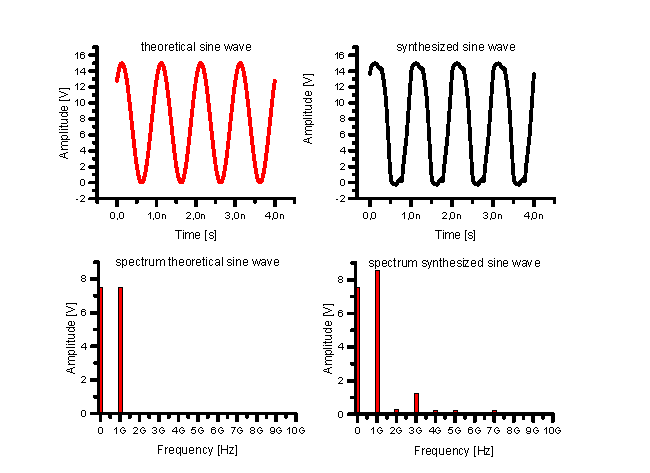
\includegraphics[width=1\textwidth]{SineCompare.pdf}
	\caption{Comparison between a theoretical and a synthesized sine wave with their spectrum}
	\label{fig:SineCompare}
\end{figure}


Figure \ref{fig:1GHz sine} shows a sine wave with a frequency of 1 GHz synthesized with the DAC. The control frequency is eight times the signal bandwidth.
\begin{figure}[htb!]
   \centering
   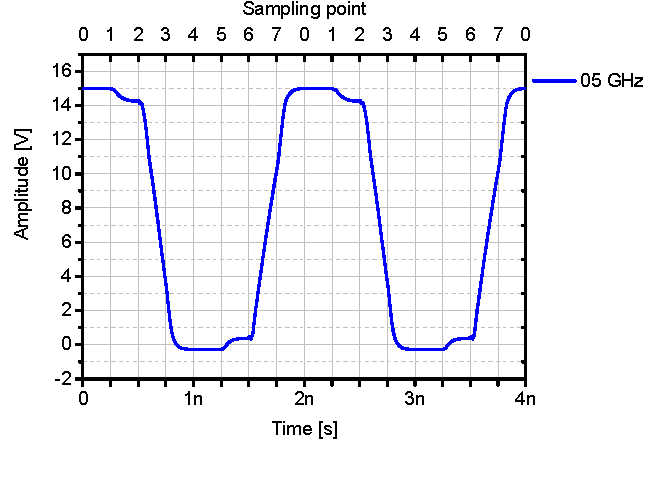
\includegraphics[width=0.75\textwidth]{Vout_sine_SigBW_05GHz_3bit_long.pdf}
   \caption{amplitude of a synthesized sine wave with signal frequency of 500 MHz, $f_{sampling} =$ \SI{4}{\GHz} in the time domain}
   \label{fig:05GHz sine}
\end{figure}
\begin{figure}[htb!]
   \centering
   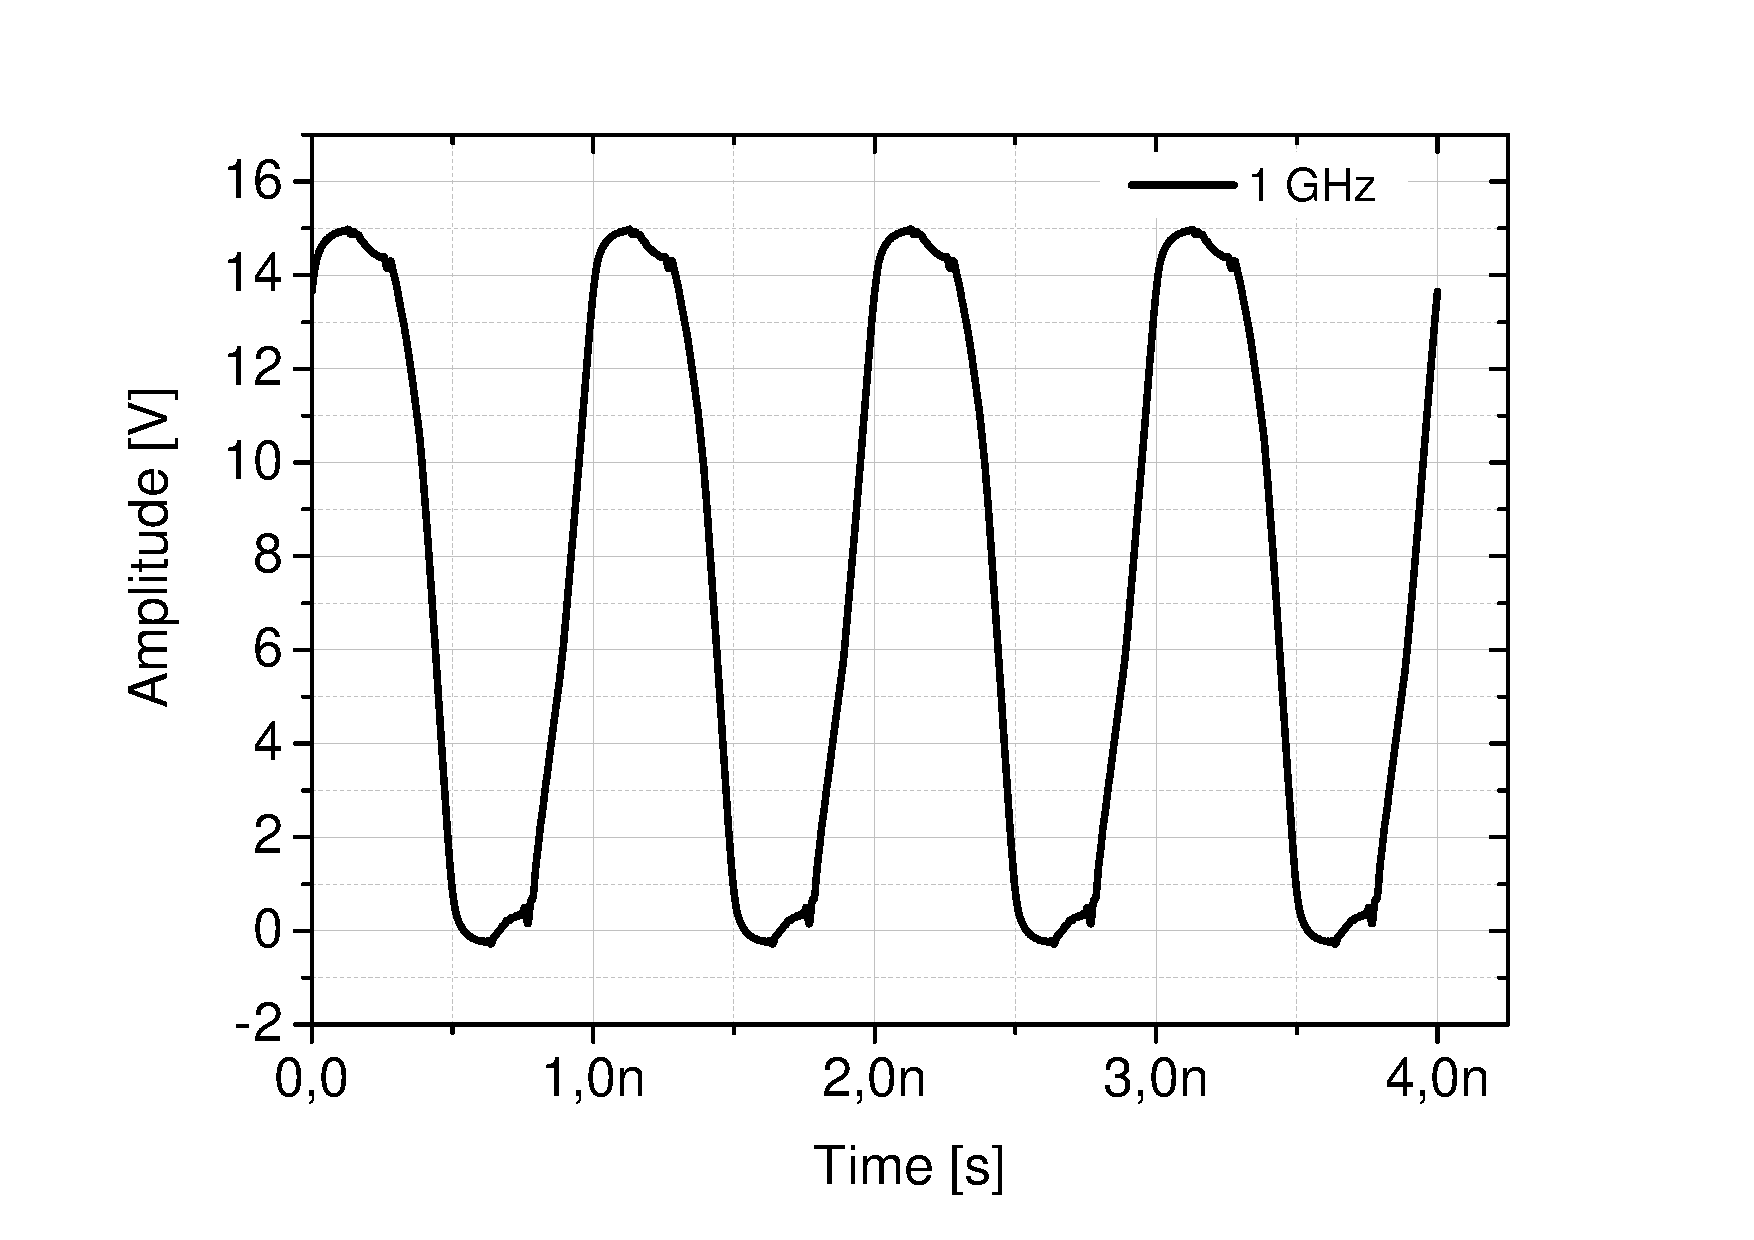
\includegraphics[width=0.75\textwidth]{Vout_sine_SigBW_1GHz_3bit_long.pdf}
   \caption{amplitude of a synthesized sine wave with signal frequency of 1 GHz, $f_{sampling} =$ \SI{8}{\GHz} in the time domain}
   \label{fig:1GHz sine}
\end{figure}
\begin{figure}[htb!]
   \centering
   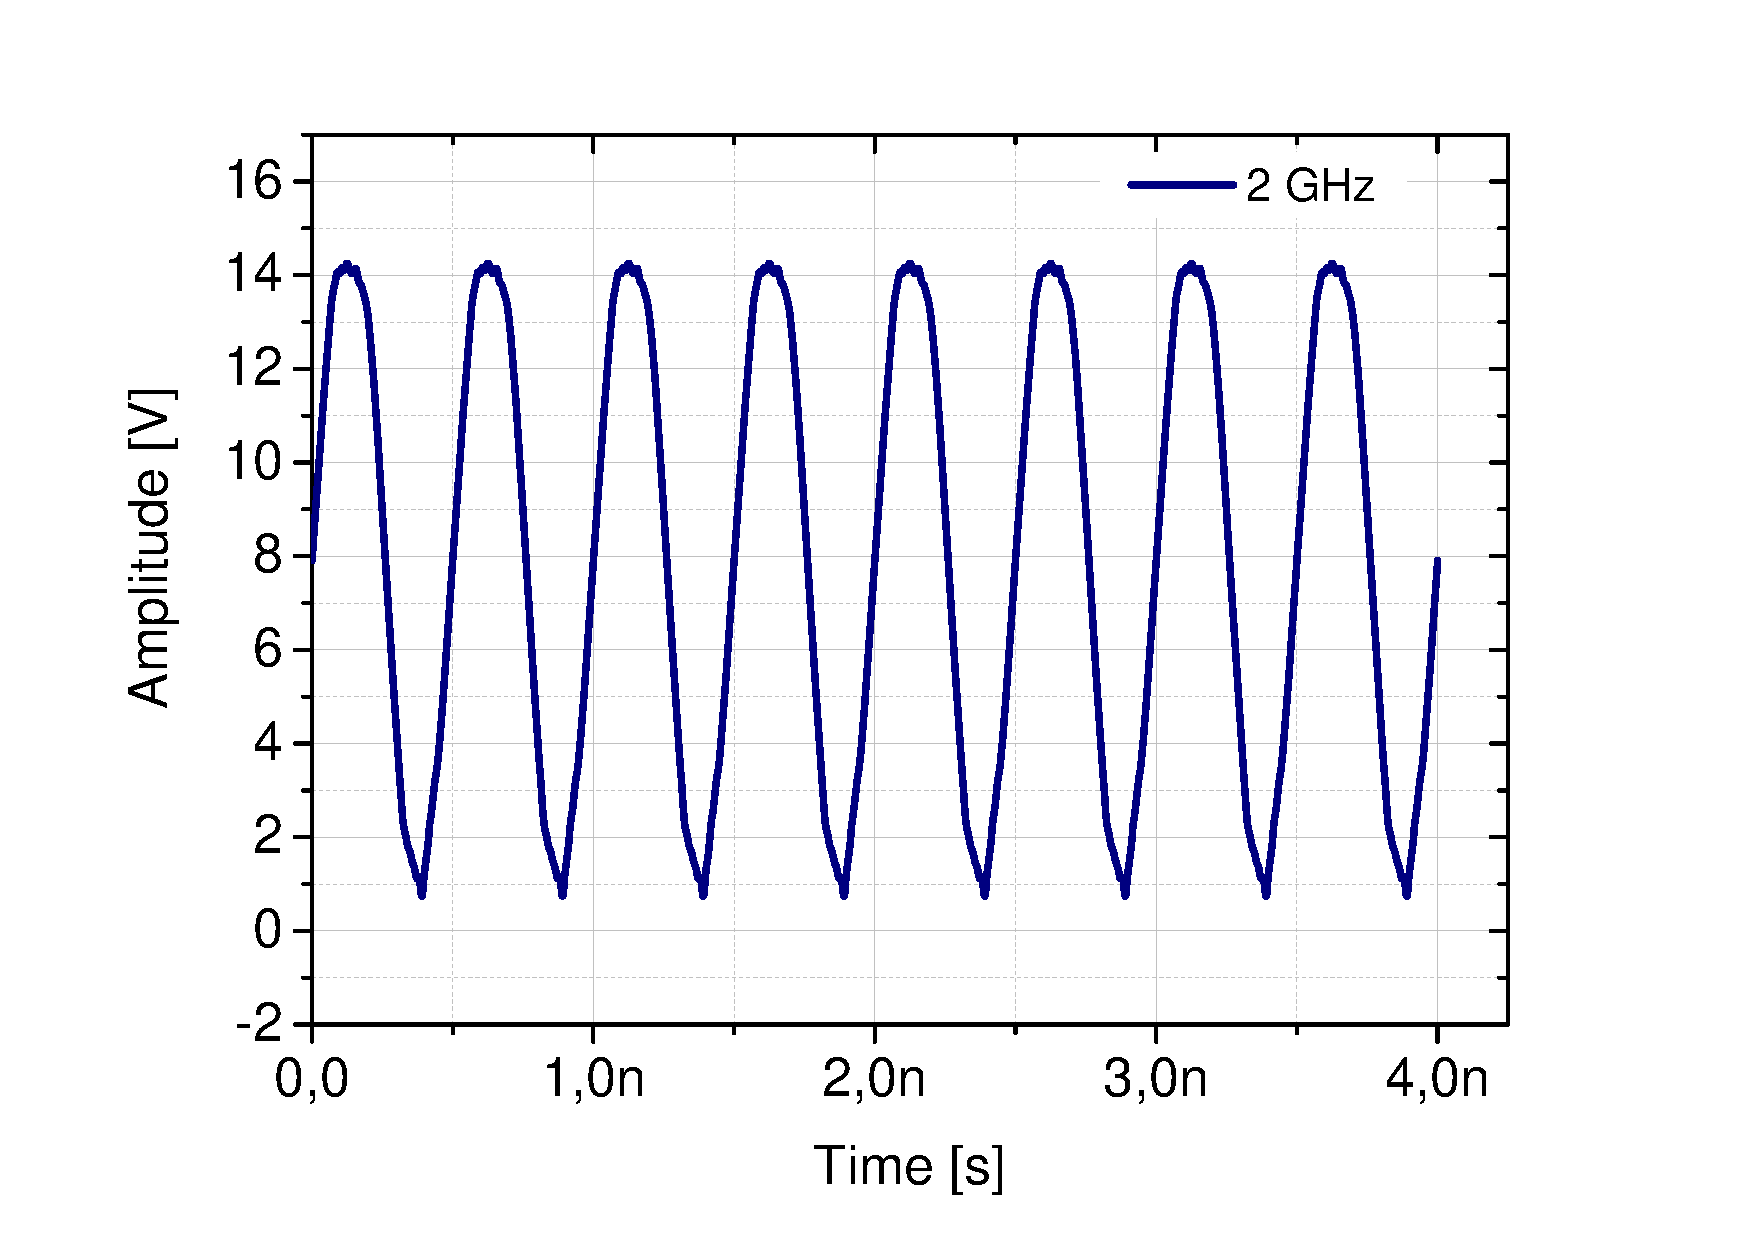
\includegraphics[width=0.75\textwidth]{Vout_sine_SigBW_2GHz_3bit_long.pdf}
   \caption{amplitude of a synthesized sine wave with signal frequency of 2 GHz, $f_{sampling} =$ \SI{16}{\GHz} in the time domain}
   \label{fig:2GHz sine}
\end{figure}




This signal is generated with the riemann code. This riemann code was obtained by hand with optical estimation with the slopes obtained from the table.
\subsection{half sine}
Based on the same optical approximation of the signal in Fig. \ref{fig:SineWaveCodeGeneration} the riemanncode for the half sine is generated. The Riemanncode for the half sine is: 000 010 101 111 000 010 101 111
\subsection{triangular}
This is a triangular wave.


\section{Time signal simulation with component dimension like demonstrator}
This two bit resolution simulation is done to compare the demonstrators measurements with the simulation. \textbf{two-bit resolution, osr = 4, keep it small and simple, frequency higher, demonstrator, assembly, less complex} 
The three bit resolution DAC was too complex to realize in a first approach on a hybrid substrate
\subsection{differences of three signals which can be compared to measurements}
Here to present the two bit resolution sine wave, half sine wave and triangular



\section{Stability analysis}
Stability simulation is done to check whether or not oscillation occurs.
A stability analysis is done within the ADS tool. This should state that the corresponding circuit do not oscillate at specific frequencies or frequency ranges.

\section{Energy consumption analysis}
\textbf{switch voltage for on off state} switch time, static losses and dynamic losses.
The energy consumption is analysed with the circuit created by me in ADS. For the chips used for the demonstrator refer to the work of Stephan Maroldt who states, that the power consumption is:  divided into static and dynamic ones. The switching losses are greater than the static ones.
